%%%%%%%%%%%%
%
% $Autor: Zarzycki $
% $Datum: 2025-09-26 11:30:00Z $
% $Pfad: TemplateSensor $
% $Version: 4250 $
% !TeX spellcheck = en_GB/de_DE
% !TeX encoding = utf8
% !TeX root = filename 
% !TeX TXS-program:bibliography = txs:///biber
%
%%%%%%%%%%%%

\chapter{LoRa \label{lora:general}}
	Dieses Kapitel beschreibt die physikalischen Grundlagen der \acf{lora}-Modulation, einschlie{\ss}lich Spreading Factor, Bandbreite, Coding Rate und deren Einfluss auf Reichweite, Datenrate und Robustheit. Es erläutert zentrale Leistungsparameter wie Sendeleistung, Empfindlichkeit, RSSI, SNR und Link-Budget, sowie regulatorische Aspekte wie Duty-Cycle-Beschränkungen im EU-Frequenzband. Zusätzlich wird das Funktionsprinzip der Chirp-Spread-Spectrum-Modulation, der Aufbau eines \acs{lora}-Pakets und die Demodulation mittels Dechirping und schnelle Fourier-Transformation (FFT) dargestellt.
	
\section{Einleitung}
	\acf{lora} ist eine Funktechnologie, die speziell für eine energieeffiziente Datenübertragung über gro{\ss}e Distanzen entwickelt wurde \cite{Semtech:2015}. Sie gehört zur Familie der LPWAN-Technologien (Low Power Wide Area Networks) und ermöglicht Kommunikation mit sehr geringer Datenrate bei minimalem Energieverbrauch \cite{Semtech:2024}.	
	In der Fachliteratur und innerhalb der Industrie bestehen unterschiedliche Auffassungen über die genaue Abgrenzung zwischen \textit{LoRa\texttrademark} und \textit{LoRaWAN\texttrademark}. Silver Spring Networks (UK) weist in \textcite{ETSI:2018} darauf hin, dass \textit{LoRa} die physikalische Schicht bzw. Modulation zur Realisierung der Langstreckenverbindung darstellt, während \textit{LoRaWAN} das Kommunikationsprotokoll und die Netzwerkarchitektur beschreibt.\textcite{Semtech:2024} nennt eine Reichweite für LoRa von bis zu 5 km in urbanen Gebieten und bis zu 15 km oder mehr in ländlichen Gebieten. Auch die Akkulaufzeit wird laut Semtech mit bis zu zehn Jahren angegeben.
	
	\vspace{0.5cm}
	LoRa basiert auf der \textit{Chirp Spread Spectrum}-Modulation (CSS) (siehe~\ref{lora:modulation}), bei der das Signal durch eine kontinuierliche Änderung der Trägerfrequenz (\textit{chirp}) über eine definierte Bandbreite verteilt wird. Die Technologie verwendet variable Datenraten und orthogonale \textit{Spreading Factors (SF)} (siehe~\ref{lora:sf}), die es ermöglichen, das Verhältnis zwischen Datenrate, Reichweite und Energieverbrauch flexibel anzupassen. \cite{Semtech:2015}.


	\begin{figure}[H]
		\centering
		\begin{tikzpicture}
			\protocolsiot
		\end{tikzpicture}
		\caption{Vergleich verschiedener Funktechnologien hinsichtlich Bandbreite und Reichweite. \cite{Montagny:2022}}
	\end{figure}

\section{Spreading Factor (SF) \label{lora:sf}}
	
	Der \textbf{Spreading Factor (SF)} ist ein zentraler Parameter der \textit{Chirp Spread Spectrum} (CSS) - Modulation von LoRa. Er bestimmt die Steigung und die zeitliche Länge der einzelnen \textit{Chirps} \cite{ETSI:2018}. Der SF-Wert liegt typischerweise im Bereich von 7 bis 12 und muss vor der Übertragung sowohl auf der Sender- als auch auf der Empfängerseite bekannt sein \cite{Semtech:2015b}. Je höher der Spreading Factor, desto länger dauert die Übertragung eines Symbols, was zu einer geringeren Datenrate, aber zu einer höheren Empfindlichkeit und Reichweite führt \cite{Montagny:2022}. Ein höherer SF ermöglicht also eine robustere Kommunikation über grö{\ss}ere Distanzen, während ein niedriger SF eine höhere Datenrate auf Kosten der Reichweite erlaubt \cite{Savaux:2021}.
		
	\begin{table}[H]
		\centering
		\caption{Chirp-Dauer als Funktion des Spreading Factors}
		\begin{tabular}{c|c}
			\textbf{Spreading Factor (SF)} & \textbf{Chirp-Dauer [ms]} \\ \hline
			7 & 1 \\
			8 & 2 \\
			9 & 4 \\
			10 & 8 \\
			11 & 16 \\
			12 & 32 \\
		\end{tabular}
	\end{table}
	
\begin{figure}[H]
	\centering
	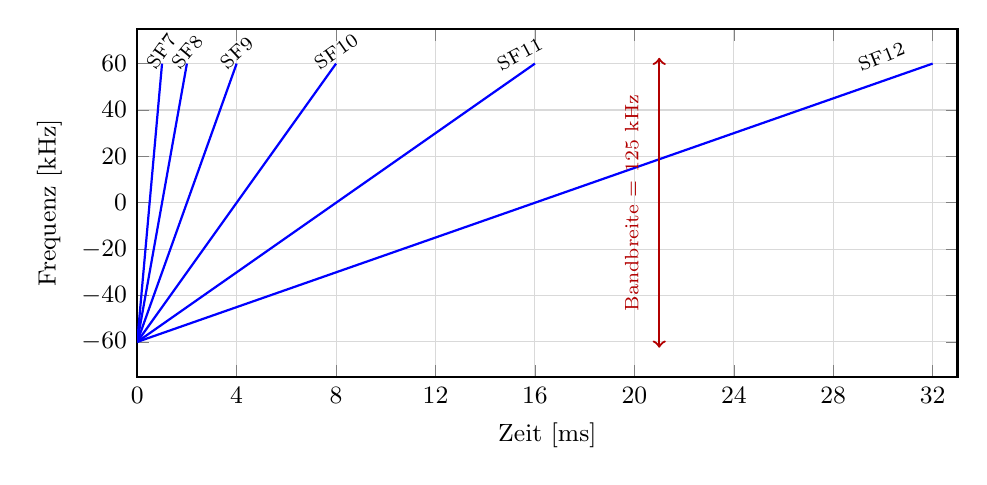
\begin{tikzpicture}
		\tikzset{
			textLabel/.style={
				font=\scriptsize,
				above right,
				text opacity=1,
				fill opacity=0,
				inner sep=5pt,
				pos=0.9,
				color=black
			},
			lineStyle/.style={color=blue},
			bandLabel/.style={
				font=\scriptsize,
				color=red!70!black
			}
		}
		\begin{axis}[
			width=12cm,
			height=6cm,
			xlabel={Zeit [ms]},
			ylabel={Frequenz [kHz]},
			xmin=0, xmax=33,
			ymin=-75, ymax=75,
			xtick={0,4,8,12,16,20,24,28,32},
			ytick={-60,-40,-20,0,20,40,60},
			grid=both,
			every major grid/.style={gray!30},
			line width=0.8pt,
			tick label style={font=\small},
			label style={font=\small},
			]
			
			% --- SF7 bis SF12 ---
			\addplot[lineStyle, thick, domain=0:1] {120*x - 60}
			node[textLabel, rotate=55]{SF7};
			
			\addplot[lineStyle, thick, domain=0:2] {60*x - 60}
			node[textLabel, rotate=50]{SF8};
			
			\addplot[lineStyle, thick, domain=0:4] {30*x - 60}
			node[textLabel, rotate=43]{SF9};
			
			\addplot[lineStyle, thick, domain=0:8] {15*x - 60}
			node[textLabel, rotate=35]{SF10};
			
			\addplot[lineStyle, thick, domain=0:16] {7.5*x - 60}
			node[textLabel, rotate=28]{SF11};
			
			\addplot[lineStyle, thick, domain=0:32] {3.75*x - 60}
			node[textLabel, rotate=22]{SF12};
			
			% --- Bandbreite ---
			\draw[<->, red!70!black, thick] (axis cs:21,-62.5) -- (axis cs:21,62.5)
			node[midway, bandLabel, rotate=90, yshift=1em]{Bandbreite = 125 kHz};
			
		\end{axis}
	\end{tikzpicture}
	\caption{Darstellung der Frequenzänderung von $-62{,}5$\,kHz bis $+62{,}5$\,kHz 
		innerhalb einer Bandbreite von 125\,kHz für verschiedene Spreading Factors (SF). 
		Ein höherer SF führt zu einer flacheren Steigung und somit zu einer längeren Symbolzeit.}
\end{figure}


	
	
	\begin{figure}[H]
		\centering
		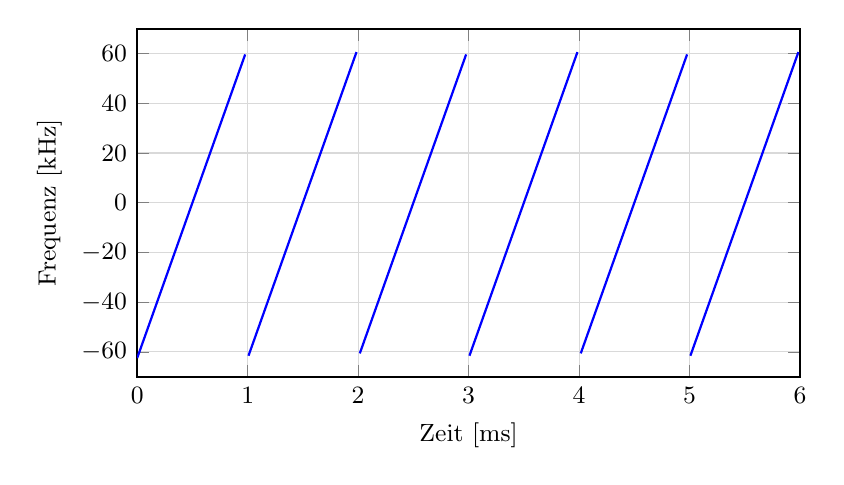
\begin{tikzpicture}
			\begin{axis}[
				width=10cm,
				height=6cm,
				xlabel={Zeit [ms]},
				ylabel={Frequenz [kHz]},
				xmin=0, xmax=6,
				ymin=-70, ymax=70,
				xtick={0,1,2,3,4,5,6},
				ytick={-60,-40,-20,0,20,40,60},
				grid=both,
				every major grid/.style={gray!30},
				line width=0.8pt,
				tick label style={font=\small},
				label style={font=\small},
				unbounded coords=jump
				]
				% Chirp signal: linear sweep repeating every 1 ms
				\addplot[blue, thick, samples=400, domain=0:6]
				{ (mod(125*x,125) < 124) ? (mod(125*x,125) - 62.5) : nan };
			\end{axis}
		\end{tikzpicture}
		\caption{Verlauf der momentanen Frequenz eines LoRa-Up-Chirps mit einer Bandbreite von 125~kHz und einem Spreading Factor von 7 (Chirp-Dauer 1~ms).}
	\end{figure}
	
	
	\begin{figure}[H]
		\centering
		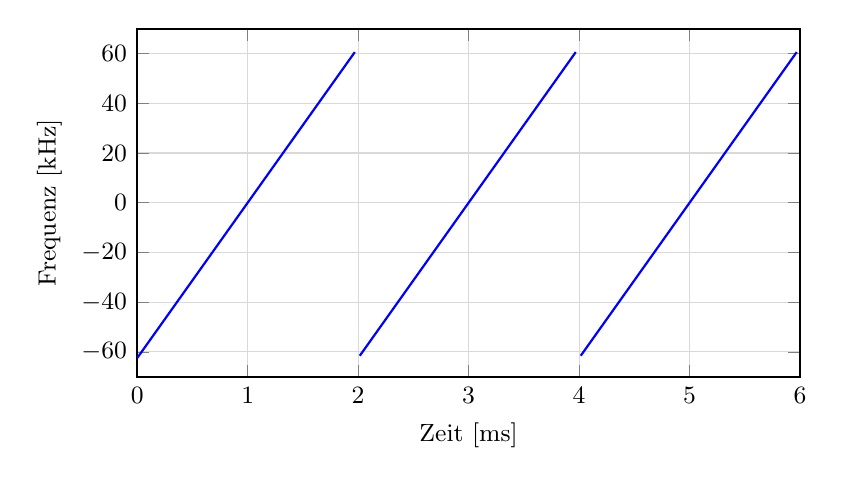
\begin{tikzpicture}
			\begin{axis}[
				width=10cm,
				height=6cm,
				xlabel={Zeit [ms]},
				ylabel={Frequenz [kHz]},
				xmin=0, xmax=6,
				ymin=-70, ymax=70,
				xtick={0,1,2,3,4,5,6},
				ytick={-60,-40,-20,0,20,40,60},
				grid=both,
				every major grid/.style={gray!30},
				line width=0.8pt,
				tick label style={font=\small},
				label style={font=\small},
				unbounded coords=jump
				]
				% Chirp signal: linear sweep repeating every 2 ms
				\addplot[blue, thick, samples=400, domain=0:6]
				{ (mod(125*(x/2),125) < 124) ? (mod(125*(x/2),125) - 62.5) : nan };
			\end{axis}
		\end{tikzpicture}
		\caption{Verlauf der momentanen Frequenz eines LoRa-Up-Chirps mit einer Bandbreite von 125~kHz und einem Spreading Factor von 8 (Chirp-Dauer 2~ms).}
	\end{figure}
	
	\subsection{Orthogonalität \label{lora:orthogonal}}
	Ein besonderes Merkmal der LoRa-Modulation besteht darin, dass Signale mit unterschiedlichen Spreading Factors \textbf{orthogonal} zueinander sind, was sich auf eine geringe Kreuzkorrelation dieser Signale bezieht \cite{Semtech:2015, Semtech:2015b, Vangelista:2017}. Wenn sich solche Signale überlagern oder zusammen addieren, interferieren sie nicht miteinander. Dies bedeutet, dass mehrere Geräte gleichzeitig auf derselben Frequenz senden können, ohne sich gegenseitig wesentlich zu stören. Ein Empfänger kann überlagerte Signale mit verschiedenen SF-Werten gleichzeitig demodulieren, sofern eine ausreichende Leistungsreserve ($SNR_{margin}$) zwischen ihnen besteht \cite{ETSI:2018}. 
	Diese Eigenschaft trägt wesentlich zur hohen Kanalnutzungseffizienz von LoRa bei, da mehrere Endgeräte gleichzeitig im selben Frequenzkanal aktiv sein können \cite{Montagny:2022}.
	
	
	
	\begin{figure}[h!]
		\centering
		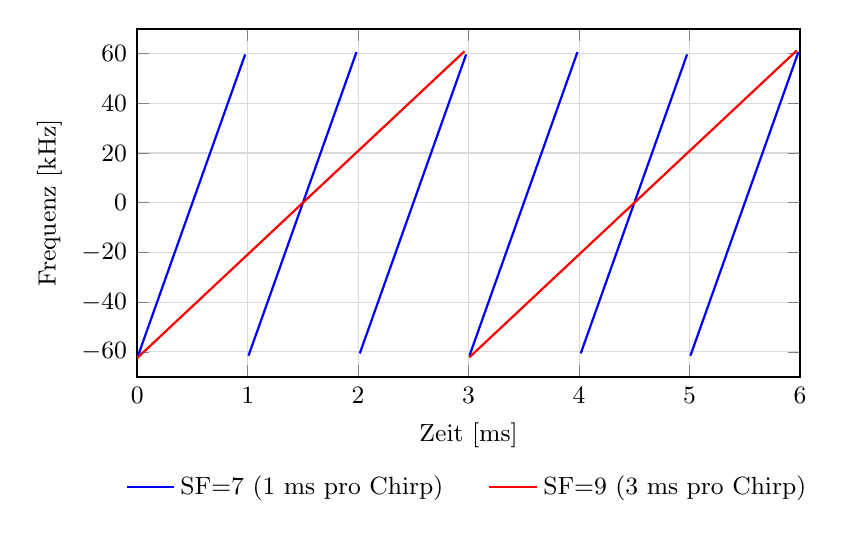
\begin{tikzpicture}
			\begin{axis}[
				width=10cm,
				height=6cm,
				xlabel={Zeit [ms]},
				ylabel={Frequenz [kHz]},
				xmin=0, xmax=6,
				ymin=-70, ymax=70,
				xtick={0,1,2,3,4,5,6},
				ytick={-60,-40,-20,0,20,40,60},
				grid=both,
				every major grid/.style={gray!30},
				line width=0.8pt,
				tick label style={font=\small},
				label style={font=\small},
				unbounded coords=jump,
				legend style={
					at={(0.5,-0.25)},
					anchor=north,
					font=\small,
					draw=none,
					fill=none,
					legend columns=-1,
					/tikz/every even column/.append style={column sep=0.5cm}
				}
				]
				\addplot[blue, thick, samples=400, domain=0:6]
				{ (mod(125*x,125) < 124) ? (mod(125*x,125) - 62.5) : nan };
				\addlegendentry{SF=7 (1~ms pro Chirp)}
				
				\addplot[red, thick, samples=400, domain=0:6]
				{ (mod(125*(x/3),125) < 124) ? (mod(125*(x/3),125) - 62.5) : nan };
				\addlegendentry{SF=9 (3~ms pro Chirp)}
			\end{axis}
		\end{tikzpicture}
		\caption{Vergleich der momentanen Frequenzen zweier LoRa-Up-Chirps mit einer Bandbreite von 125~kHz und unterschiedlichen Spreading Factors.}
	\end{figure}
	
\subsection{Anzahl der Bits pro Symbol}

	Der \textbf{Spreading Factor (SF)} definiert, wie viele Bits ein Symbol repräsentieren. Ein Symbol in LoRa besteht aus \( SF \) Informationsbits, was bedeutet, dass es insgesamt \( 2^{SF} \) verschiedene Symbolzustände geben kann.
	
	\[
	\text{Anzahl der möglichen Symbole} = 2^{SF}
	\]
	
	Zum Beispiel repräsentiert ein Symbol bei \( SF = 10 \) insgesamt \( 2^{10} = 1024 \) mögliche Zustände und damit 10 Bits Information. Diese Zustände werden durch unterschiedliche \textit{Chirps} (zeitlich frequenzmodulierte Signale) dargestellt.

	\begin{table}[H]
		\centering
		\caption{Zusammenhang zwischen Spreading Factor, Informationsbits und möglichen Symbolzuständen}
		\begin{tabular}{c|c|c}
			\hline
			\textbf{Spreading Factor (SF)} & \textbf{Bits pro Symbol} & \textbf{Mögliche Zustände ($2^{SF}$)} \\ \hline
			7  & 7  & 128 \\
			8  & 8  & 256 \\
			9  & 9  & 512 \\
			10 & 10 & 1024 \\
			11 & 11 & 2048 \\
			12 & 12 & 4096 \\ \hline
		\end{tabular}
	\end{table}
	
\subsection{Einfluss des Spreading Factors auf die Signalrobustheit}

	Ein grö{\ss}erer \textbf{Spreading Factor (SF)} führt dazu, dass ein Symbol durch einen einzigen, aber zeitlich verlängerten \textit{Chirp} dargestellt wird. Dabei repräsentiert jedes Symbol \(SF\) Informationsbits, was bedeutet, dass bei höherem SF ein Symbol aus mehr Bits besteht \cite{ETSI:2018}. 
	
	Dies erhöht die Robustheit der Übertragung: Der Empfänger kann das Symbol auch dann noch korrekt rekonstruieren, wenn Teile des Signals durch Rauschen oder Interferenzen gestört sind. Mit zunehmendem SF steigt somit die \textbf{Empfindlichkeit} und die \textbf{Reichweite} der Übertragung, während die \textbf{Datenrate} abnimmt \cite{Semtech:2015}. 

\section{Bitrate, Symbolrate und Coding Rate}
	\textcite{Semtech:2015} weist darauf hin, dass die \textbf{Bitrate}, \textbf{Symbolrate} und \textbf{Coding Rate} miteinander verknüpft sind. Eine Änderung des \textbf{\hyperref[lora:sf]{Spreading Factors (SF)}} oder der \textbf{\hyperref[lora:bandWidth]{Bandbreite}} kann dabei einzelne Parameter verschlechtern, während andere verbessert werden.
	
\subsection{Bitrate}
	Die \textbf{Bitrate} beschreibt, wie viele Bits pro Sekunde übertragen werden können. In \ac{lora} hängt sie von drei physikalischen Parametern ab:
	\begin{itemize}
		\item Bandbreite (BW)
		\item Spreading Factor (SF)
		\item Coding Rate (CR)
	\end{itemize}
	
	\[
	R_b = SF \times \frac{BW}{2^{SF}} \times CR
	\]
	
	Mit zunehmendem \textbf{Spreading Factor} verlängert sich die Symbolzeit, wodurch die Bitrate abnimmt, die Reichweite und Empfindlichkeit jedoch steigen. Eine grö{\ss}ere \textbf{Bandbreite} führt zu einer höheren Datenrate, reduziert aber die Empfindlichkeit des Empfängers \cite{Semtech:2024}. Die \textbf{Coding Rate} bestimmt das Verhältnis zwischen Nutz- und Redundanzbits: eine niedrigere CR (z.\,B.\ 4/5) erhöht die Datenrate, verringert jedoch die Fehlertoleranz (siehe~\ref{lora:codingRate}).
	
	\subsection{Symbolrate \label{lora:symbolRate}}
	Die \textbf{Symbolrate} gibt an, wie viele Symbole pro Sekunde übertragen werden können. 
	Sie wird durch die Bandbreite und den Spreading Factor bestimmt und kann folgenderma{\ss}en berechnet werden:
	\[
	R_s = \frac{BW}{2^{SF}} \quad \left[\frac{\text{Symbole}}{\text{Sekunde}}\right]
	\]
	
	\subsubsection{Symbolzeit \label{lora:symbolTransmissionTime}}
	Die \textbf{Symbolzeit} \(T_s\) beschreibt die Dauer eines einzelnen Symbols, also die Zeit, die benötigt wird, um ein Symbol vollständig zu übertragen. Sie ist der Kehrwert der Symbolrate und hängt direkt vom Spreading Factor und von der verwendeten Bandbreite ab. Je höher der Spreading Factor, desto länger dauert die Übertragung eines Symbols, wodurch die Datenrate sinkt, aber die Empfindlichkeit und Reichweite der Übertragung steigen \cite{Montagny:2022}. 
	
	\[
	T_s = \frac{2^{SF}}{BW}~\text{sek}
	\]

	
	\subsection{Coding Rate \label{lora:codingRate}}
	LoRa implementiert ein \textbf{Vorwärtsfehlerkorrekturschema (Forward Error Correction, FEC)}, das die Robustheit des übertragenen Signals auf Kosten einer zusätzlichen Redundanz erhöht. Dabei wird jedem Nutzdatenbit eine bestimmte Anzahl an Redundanzbits hinzugefügt, um Übertragungsfehler auf Empfängerseite erkennen und teilweise korrigieren zu können.
	
	Die \textbf{Coding Rate (CR)} beschreibt das Verhältnis zwischen den tatsächlich übertragenen Bits und den Nutzdatenbits. Sie wird nach folgender Formel berechnet:
	\[
	\text{CR} = \frac{4}{4 + N}
	\]
	wobei \(N\) den Wert zwischen 1 und 4 annehmen kann und die Stärke der Fehlerkorrektur angibt.
	
	Typische Werte sind:
	\[
	N = 1 \Rightarrow \text{CR} = \frac{4}{5}, \quad
	N = 2 \Rightarrow \text{CR} = \frac{4}{6}, \quad
	N = 3 \Rightarrow \text{CR} = \frac{4}{7}, \quad
	N = 4 \Rightarrow \text{CR} = \frac{4}{8}.
	\]
	
	Ein niedrigerer Wert (z.\,B.\ \(\text{CR} = 4/5\)) führt zu einer höheren Datenrate, da weniger Redundanz übertragen wird, ist jedoch weniger robust gegenüber Rauschen und Störungen. Ein höherer Wert (z.\,B.\ \(\text{CR} = 4/8\)) verbessert die Fehlertoleranz und die Reichweite, verringert jedoch die effektive Bitrate \cite{Montagny:2022}.


\section{Bandbreite (BW) \label{lora:bandWidth}}
	Die \textbf{Bandbreite (BW)} beschreibt den Frequenzbereich, in dem ein Funksignal eine signifikante Energie aufweist \cite{ETSI:2017}. Sie wird in Hertz angegeben und bestimmt die spektrale Ausdehnung des Signals. Im Allgemeinen entspricht sie der Differenz zwischen der höchsten und der niedrigsten genutzten Frequenz (\(BW = f_\text{max} - f_\text{min}\)) \cite{ETSI:2017}.
	
	\begin{figure}[H]
		\centering
		\begin{tikzpicture}[>=stealth, scale=1.2]
			
			% Oś częstotliwości
			\draw[thick, ->] (0,0) -- (7,0) node[right]{\textbf{Frequenz}};
			
			% Prostokąt pasma
			\draw[thick, fill=gray!30] (2,0) -- (2,1.2) -- (5,1.2) -- (5,0) -- cycle;
			\draw[thick, dashed, blue] (3.5, 0) -- (3.5, 1.2);
			
			% Strzałka zakresu pasma
			\draw[<->, thick, blue] (2,1.5) -- (5,1.5)
			node[midway, above]{\textbf{Bandbreite}};
			
			% Opisy częstotliwości
			\node[below] at (2,0) {\small{$f_\text{min}$}};
			\node[below] at (3.5,0) {\small{$f_\text{Träger}$}};
			\node[below] at (5,0) {\small{$f_\text{max}$}};
			\end{tikzpicture}
		\caption{Schematische Darstellung der Bandbreite um die Trägerfrequenz \(f_c\) \cite{Montagny:2022}}
	\end{figure}
	
	Dabei sind \(f_\text{min}\) und \(f_\text{max}\) durch \(f_c \pm \frac{BW}{2}\) definiert, wobei \(f_c\) die Trägerfrequenz darstellt \cite{Montagny:2022}. 
	
	
	In der \hyperref[lora:modulation]{\textit{Chirp Spread Spectrum} (CSS) - Modulation} legt die Bandbreite fest, wie weit die Frequenz eines Chirps während eines Symbols variiert \cite{Semtech:2015}. Eine grö{\ss}ere Bandbreite bedeutet, dass der Chirp den Frequenzbereich schneller durchläuft, was zu kürzeren Symbolzeiten und somit zu einer höheren Übertragungsgeschwindigkeit führt:
	\[
	T_s = \frac{2^{SF}}{BW}~\text{sek}
	\]
	wobei \(T_s\) die Symbolperiode bezeichnet (siehe~\autoref{lora:symbolTransmissionTime}). Dies wirkt sich direkt auf die \hyperref[lora:symbolRate]{Symbolrate} aus:
	\[
	R_s = \frac{1}{T_s} = \frac{BW}{2^{SF}} \quad \left[\frac{\text{Symbole}}{\text{sekunde}}\right]
	\]
	Gleichzeitig wird jedoch ein breiteres Rauschband erfasst, was die Empfindlichkeit des Empfängers verringert und die maximale Kommunikationsreichweite reduziert. Dieser Zusammenhang lässt sich durch die Gleichung
	\[
	P_\text{min} = -174 + 10\log_{10}(BW) + NF + SNR_\text{min}
	\]
	beschreiben, wobei \(NF\) den Rauschfaktor und \(SNR_\text{min}\) das minimale erforderliche Signal-Rausch-Verhältnis darstellen (siehe~\ref{lora:sensitivity}). Eine kleinere Bandbreite bewirkt das Gegenteil: Die Frequenzänderung innerhalb eines Symbols erfolgt langsamer, die Symbole dauern länger, und die Übertragungsgeschwindigkeit sinkt. Dafür verbessert sich jedoch die \hyperref[lora:snr]{Signal-zu-Rausch-Verhältnis}, was schwächere Signale und somit grö{\ss}ere Reichweiten ermöglicht.
	
	Die Wahl der Bandbreite stellt daher einen zentralen Kompromiss dar: Eine hohe Bandbreite ermöglicht schnelle, aber weniger empfindliche Übertragungen, während eine schmale Bandbreite eine höhere Robustheit und Reichweite auf Kosten der Datenrate bietet \cite{Semtech:2015}.
	
	
	\begin{table}[H]
		\centering
		\caption{Einfluss der Bandbreite auf Systemparameter}
		\begin{tabular}{l|c|c|c}
			\textbf{Bandbreite} & \textbf{Datenrate} & \textbf{Reichweite} & \textbf{Empfindlichkeit} \\ \hline
			125~kHz & mittel & hoch & gut \\
			250~kHz & hoch & mittel & reduziert \\
			500~kHz & sehr hoch & gering & schwach \\
		\end{tabular}
	\end{table}

\section{Sendeleistung, Empfindlichkeit und Link Budget}
	\subsection{Dezibel (dB) \label{lora:decibel}}	
	Um die Begriffe \textbf{Sendeleistung} und \textbf{Empfindlichkeit} richtig verstehen zu können, muss zunächst erläutert werden, was unter einem \textbf{Dezibel (dB)} zu verstehen ist. Der Dezibelwert (dB) ist eine logarithmische Ma{\ss}einheit, die das Verhältnis zwischen zwei Leistungs- oder Spannungsgrö{\ss}en beschreibt. Er wird häufig verwendet, um Signalstärken oder Dämpfungen darzustellen, da gro{\ss}e Wertebereiche dadurch kompakt ausgedrückt werden können. Als Verhältnis zwischen Ausgangs- und Eingangsgrö{\ss}e ist der Dezibelwert ein einheitenloses, relatives Ma{\ss} und beschreibt den Verstärkungsfaktor \cite[337-339]{Stiny:2024}.
	
	Die Spannungsverstärkung in Dezibel wird definiert als:
	\[
	L_\text{dB} = 20 \log_{10}\!\left(\frac{U_2}{U_1}\right)
	\]
	
	Für die Leistungsverstärkung gilt entsprechend:
	\[
	L_\text{dB} = 10 \log_{10}\!\left(\frac{P_2}{P_1}\right)
	\]
	Positive Ergebnisse bedeuten Verstärkung, negative Werte Dämpfung.
	
	\vspace{0.5cm}
	
	Neben dem allgemeinen Dezibelbegriff werden in der Funktechnik häufig abgeleitete Einheiten (\cite{ETSI:2018}) verwendet:
	\begin{itemize}
		\item \textbf{dBm} beschreibt eine absolute Leistung, bezogen auf eine Referenzleistung von 1 milliwatt. Damit entspricht beispielsweise 0 dBm genau 1 milliwatt Sendeleistung.
		\item \textbf{dBi} gibt den Antennengewinn im Vergleich zu einer idealen isotropen Antenne an, die ihre Leistung gleichmä{\ss}ig in alle Richtungen abstrahlt.
		\item \textbf{dBd} bezieht sich auf den Antennengewinn gegenüber einem idealen Dipol als Referenzantenne. Zwischen beiden Grö{\ss}en besteht der Zusammenhang:
		\[
		dBi=dBd+2,15
		\]
	\end{itemize}

	\subsubsection{Beispiel}
	Gegeben seien eine Eingangsleistung von $P_1 = 2~\text{mW}$	und eine Ausgangsleistung von $P_2 = 20~\text{mW}$.
	Die Leistungsverstärkung beträgt somit:
	\[
	L_\text{dB} = 10 \log_{10}\!\left(\frac{P_2}{P_1}\right)
	= 10 \log_{10}\!\left(\frac{20}{2}\right)
	= 10 \log_{10}(10)
	= 10~\text{dB}.
	\]
	Damit beträgt die Verstärkung \textbf{10 dB}.
	
	
	\subsection{Sendeleistung \label{lora:txpower}}
	Die \textbf{Sendeleistung} beschreibt die vom Sender abgegebene Leistung, die in Richtung des Empfängers übertragen wird. Um gro{\ss}e Wertebereiche kompakt darzustellen, wird sie ebenfalls in Dezibel angegeben. Dabei wird die Leistung auf 1~mW bezogen, wodurch sich die Einheit dBm ergibt (\cite{Montagny:2022}):
	\[
	P_\text{dBm} = 10 \log_{10}\!\left(\frac{P}{1~\text{mW}}\right)
	\]
	Eine Erhöhung der Sendeleistung um 3~dB entspricht einer Verdopplung, und eine Erhöhung um 10~dB einer Verzehnfachung der abgestrahlten Leistung. Umgekehrt bedeutet eine Verringerung um 3~dB eine Halbierung und um 10~dB eine Reduzierung auf ein Zehntel der ursprünglichen Leistung~\cite[15]{Seneviratne:2019}.
	
	
In Europa beträgt die maximale Stärke des emittierten Signals \textbf{+16~dBm} \cite[Abschnitt 2.4.3]{LoRaAlliance:2022}. Das bedeutet, dass die kombinierte Ausgangsleistung des Senders ($P_{TX}$) und der Antennengewinn ($G_{ant}$) diesen Wert nicht überschreiten dürfen (siehe~\ref{lora:eirp}). Bei der Berechnung müssen auch mögliche Leitungsverluste (z.\,B. durch Kabel) berücksichtigt werden.
	
	\begin{figure}[H]
		\centering
		\begin{tikzpicture}
			\transmittertx
		\end{tikzpicture}
		\caption{Darstellung des Signalpfads vom Transmitter über das Kabel bis zur Antenne \cite{TTN_EIRP_ERP}}
	\end{figure}
	
	
	\subsubsection{Äquivalente isotrope Strahlungsleistung (EIRP) \label{lora:eirp}}
	
	Die \textbf{äquivalente isotrope Strahlungsleistung (EIRP)} beschreibt die effektiv abgestrahlte Leistung 
	unter Berücksichtigung des Antennengewinns \(G_\text{ant}\) und eventueller Leitungsverluste \(L_\text{cable}\):
	\[
	P_\text{EIRP} = P_\text{TX} + G_\text{ant} - L_\text{cable}
	\]
	Sie gibt an, wie viel Leistung tatsächlich in Richtung des grö{\ss}ten Antennengewinns abgestrahlt wird. In Europa beträgt der zulässige Maximalwert nach ETSI-Richtlinie \textbf{+16~dBm}, was einer effektiven Sendeleistung von etwa 40~mW entspricht \cite[Abschnitt 2.4.3]{LoRaAlliance:2022}. Verwendet man beispielsweise eine Antenne mit +2{,}15~dBi Gewinn, darf die Ausgangsleistung des Senders \(P_\text{TX}\) höchstens +13{,}85~dBm betragen, um den Grenzwert einzuhalten.
	
	
	Der Begriff \textbf{isotrop} bezieht sich auf eine theoretische Referenzantenne, die elektromagnetische Energie vollkommen gleichmä{\ss}ig in alle Richtungen abstrahlt. Eine reale Antenne hingegen bündelt die Energie in bestimmten Richtungen und erreicht dort eine höhere Feldstärke. Der Antennengewinn \(G_\text{ant}\) beschreibt, um wie viel stärker eine reale Antenne im Vergleich zu dieser idealen isotropen Antenne abstrahlt \cite[293]{Kark:2022}. Eine Antenne mit einem Gewinn von +2{,}15~dBi erzeugt somit in ihrer Hauptstrahlrichtung eine etwa 1{,}6-mal höhere Leistungsdichte als eine isotrope Antenne. Dies ergibt sich aus der Umrechnung des logarithmischen Ma{\ss}es in einen linearen Verstärkungsfaktor:
	\[
	G_\text{linear} = 10^{\frac{G_\text{dBi}}{10}} = 10^{\frac{2{,}15}{10}} \approx 1{,}64
	\]
	Die Antenne bündelt die abgestrahlte Leistung also so, dass in ihrer Hauptstrahlrichtung rund 64~\% mehr Energie pro Fläche ankommt als bei einer isotropen Abstrahlung.
	
	\subsection{Empfindlichkeit \label{lora:sensitivity}}
	Die \textbf{Empfangsempfindlichkeit} eines Empfängers beschreibt die kleinste Signalstärke, die noch zuverlässig erkannt und dekodiert werden kann \cite{Asgharzadeh:2018}. Sie wird ebenfalls in Dezibel-Milliwatt dBm angegeben und ist ein Ma{\ss} für die Leistungsfähigkeit des Empfängers. Je niedriger der Wert, desto empfindlicher ist das Empfangssystem.
	
	Eine hohe Empfindlichkeit ermöglicht es dem Empfänger, auch sehr schwache Signale aus gro{\ss}er Entfernung oder unter schwierigen Ausbreitungsbedingungen zu erkennen. Ein LoRa-Empfänger kann unter idealen Bedingungen eine Empfindlichkeit von bis zu −142~dBm erreichen~\cite{Xu:2022b}. Typische Werte liegen jedoch bei etwa −137{,}9~dBm  (für einen Spreading Factor von 12)~\cite[Tabelle~10]{ETSI:2018}. Damit kann LoRa selbst bei sehr niedrigen \hyperref[lora:snr]{Signal-Rausch-Verhältnissen (SNR)} noch Daten zuverlässig empfangen und dekodieren.
	
	\subsubsection{Berechnung der Empfindlichkeit}
	
	Die theoretische Empfindlichkeit eines Empfängers kann mit folgender Gleichung abgeschätzt werden:
	\[
	P_\text{min} = -174 + 10\log_{10}(B) + NF + SNR_\text{min}
	\]
	mit der thermischen Rauschleistung von −174~dBm/Hz, der Bandbreite \(B\), dem \hyperref[lora:noiseFigure]{Rauschfaktor \(NF\)} und dem minimal erforderlichen \hyperref[lora:tab:snrmin]{Signal-Rausch-Verhältnissen \(SNR_\text{min}\)} \cite{ETSI:2018}.
	
	
	\subsubsection{Beispiel}
	Für eine Bandbreite von 125~kHz, einen Rauschfaktor von 6~dB und ein minimales SNR von −20~dB ergibt sich:
	\[
	P_\text{min} = -174 + 10\log_{10}(125000) + 6 - 20 \approx -130~\text{dBm}.
	\]
	Der Empfänger kann also Signale bis etwa -130~dBm noch empfangen.
	
	\subsection{Link-Budget \label{lora:linkbudget}}
	Der \textbf{Link-Budget} beschreibt die Summe aller Gewinne und Verluste, die ein Funksignal vom Sender über das Übertragungsmedium bis zum Empfänger erfährt. Er dient zur Abschätzung, ob eine Funkverbindung unter gegebenen Systemparametern realisierbar ist \cite{Semtech:2015}. Sobald die berechnete Empfangsleistung \(P_\text{RX}\) grö{\ss}er oder gleich der minimal erforderlichen Empfindlichkeit \(P_\text{min}\) (siehe~\ref{lora:sensitivity}) ist, gilt die Funkverbindung als stabil und zuverlässig \cite{PaIn:2021}. Der empfangene Signalpegel (\(P_\text{RX}\)) kann dabei wie folgt berechnet werden:
	
	\[
	P_\text{RX} = P_\text{TX} - L_\text{TX} + G_\text{TX} + G_\text{RX} - L_\text{RX} - \text{FSPL}
	\]
	
	\begin{table}[H]
		\centering
		\caption{Typische Komponenten des Link-Budgets}
		\begin{tabular}{l|c|p{6.5cm}}
			\hline
			\textbf{Parameter} & \textbf{Symbol} & \textbf{Beschreibung} \\
			\hline
			Sendeleistung & \(P_\text{TX}\) & Ausgangsleistung des Senders [dBm] \\
			Antennengewinn TX & \(G_\text{TX}\) & Richtwirkung der Sendeantenne [dBi] \\
			Antennengewinn RX & \(G_\text{RX}\) & Richtwirkung der Empfangsantenne [dBi] \\
			Verlust TX-Kabel & \(L_\text{TX}\) & Dämpfung zwischen Sender und Antenne [dB] \\
			Verlust RX-Kabel & \(L_\text{RX}\) & Dämpfung zwischen Antenne und Empfänger [dB] \\
			Pfaddämpfung & FSPL & Freiraumdämpfung in Abhängigkeit von Distanz und Frequenz [dB] (siehe~\ref{lora:fspl})\\
			Empfangsempfindlichkeit & \(P_\text{min}\) & Kleinste empfangbare Leistung [dBm] (siehe~\ref{lora:sensitivity}) \\
			\hline
		\end{tabular}
	\end{table}
	
	Hierbei gilt: Wenn \(P_\text{RX} \geq P_\text{min}\), ist die Funkverbindung stabil; liegt der Wert darunter, kommt es zu Paketverlusten oder Verbindungsabbrüchen \cite{PaIn:2021}.
	
	\subsubsection{Freiraumpfadverlust (FSPL) \label{lora:fspl}}
	\textbf{FSPL} steht für \emph{Freiraumpfadverlusts} und beschreibt die Signalverluste, die auftreten, wenn ein Signal durch den Raum übertragen wird. Je grö{\ss}er die Entfernung zwischen Sender und Empfänger ist, desto schwächer wird das Signal. Diese Verluste hängen von der Entfernung und der Frequenz des Systems ab.
	
	\[
	\text{FSPL} = 20 \log(d) + 20 \log(f) + 32{,}45
	\]
	
	wobei gilt:
	\begin{itemize}
		\item \(d\) - Entfernung zwischen den beiden Antennen [km]
		\item \(f\) - Frequenz des Signals [MHz]
		\item \(32{,}45\) -  Konstante, die sich aus der Lichtgeschwindigkeit und den verwendeten 
		Einheiten (Kilometer und Megahertz) ergibt \cite{Collins:2021}.
	\end{itemize}
	
	
	\subsubsection{Link Margin}
	Der \textbf{Link Margin} beschreibt die Leistungsreserve einer Funkverbindung. Er wird am Rand des Versorgungsgebiets bestimmt und gibt an, um wie viel die empfangene Leistung über der minimal erforderlichen Empfindlichkeit liegt (siehe~\ref{lora:sensitivity}). Ein positiver Link Margin bedeutet, dass die Verbindung stabil bleibt \cite{PaIn:2021}.
	
	
	\subsubsection{Beispiel: Empfangsleistung und Vergleich mit \(P_\text{min}\)}
	Gegeben: \(P_\text{TX} = 14~\text{dBm}\), \(G_\text{TX} = G_\text{RX} = 2~\text{dBi}\), 
	\(L_\text{TX} = L_\text{RX} = 1~\text{dB}\), \(\text{FSPL} = 130~\text{dB}\), \(P_\text{min} = -137~\text{dBm}\).
	
	\[
	P_\text{RX} = P_\text{TX} + G_\text{TX} - L_\text{TX} - \text{FSPL} - L_\text{RX} + G_\text{RX}
	\]
	
	\[
	P_\text{RX} = 14 + 2 - 1 - 130 - 1 + 2 = -114~\text{dBm}
	\]
	
	\[
	P_\text{RX} \geq P_\text{min} \Rightarrow -114~\text{dBm} > -137~\text{dBm}
	\]
	
	\[
	L_\text{Margin} = P_\text{RX} - P_\text{min} = -114~\text{dBm} - (-137~\text{dBm}) = 23~\text{dB}
	\]
	
	
	\[
	\Rightarrow \text{Verbindung stabil (Link Margin = 23~dB)}
	\]



\section{Duty Cycle}
	Der \textbf{Duty Cycle} beschreibt den Anteil der Zeit, in der ein Gerät innerhalb eines Beobachtungsintervalls aktiv senden darf. Er wird als Verhältnis oder in Prozent angegeben und dient dazu, die Auslastung des lizenzfreien ISM-Bandes zu begrenzen \cite{ETSI:2017}. 

	Gemä{\ss} dem technischen Standard \citetitle{ETSI:2018b}~(\cite{ETSI:2018b}) variiert der zulässige Duty Cycle in den europäischen ISM-Frequenzbändern je nach zugehörigem Unterband zwischen 0{,}1\,\% und 10\,\%. Für LoRa- und LoRaWAN-Anwendungen ist dabei insbesondere der Bereich 863–870\,MHz relevant, da dieser für Funkanwendungen weit verbreitet und regulatorisch klar definiert ist \cite{Montagny:2022}.

	Nach Definition der ETSI-Norm bezieht sich der Duty Cycle auf das Verhältnis der gesamten Sendezeit \(T_\text{on,cum}\) innerhalb eines Beobachtungsintervalls \(T_\text{obs}\) (typischerweise eine Stunde \cite{ETSI:2018}):
	\[
	\text{Duty Cycle} = \frac{T_\text{on,cum}}{T_\text{obs}}.
	\]
	Die Summe aller Übertragungen darf innerhalb dieses Observationsfensters den zugelassenen Anteil nicht überschreiten. Ein Endgerät kann somit mehrere Frames in kurzer Folge senden, solange der kumulierte Sendeanteil den vorgeschriebenen Duty Cycle nicht überschreitet \cite{ETSI:2017}.

\subsection{ETSI-Unterbänder und deren Beschränkungen}
	Das europäische ISM-Band ist gemä{\ss} \citeauthor[22]{ETSI:2018b} in mehrere Bänder Unterteilt, wobei sechs Unterbänder (K, L, M, N, P, Q) von Bedeutung bei LoRa und LoRaWAN andendungen sind.  Sie besitzen spezifische Beschränkungen bezüglich Duty Cycle und maximaler äquivalenter Strahlungsleistung (ERP) besitzen. Diese Vorgaben beeinflussen unmittelbar, welche Kanäle für LoRaWAN genutzt werden dürfen und wie häufig ein Gerät in diesen Bereichen senden kann.

	\begin{table}[H]
		\centering
		\begin{tabular}{|c|c|c|c|}
			\hline
			\textbf{Sub-Band} & \textbf{Frequenzbereich [MHz]} & \textbf{Duty Cycle} & \textbf{Max. ERP} \\
			\hline
			K & 863.0--865.0   & 0.1\,\%  & 25\,mW \\
			\hline
			L & 865.0--868.0   & 1\,\%    & 25\,mW \\
			\hline
			M & 868.0--868.6   & 1\,\%    & 25\,mW \\
			\hline
			N & 868.7--869.2   & 0.1\,\%  & 25\,mW \\
			\hline
			P & 869.4--869.65  & 10\,\%   & 500\,mW \\
			\hline
			Q & 869.7--870.0   & 1\,\%    & 25\,mW \\
			\hline
		\end{tabular}
		\caption{ETSI-Unterbänder im EU863--870-Band mit Duty-Cycle-Restriktionen 
			\cite{ETSI:2018b}}
	\end{table}


	Da \ac{lora} lediglich die physikalische Modulation beschreibt, muss die Einhaltung dieser gesetzlichen Duty-Cycle-Vorgaben softwareseitig durch den Entwickler bzw. das \ac{lorawan}-Endgerät sichergestellt werden. LoRa selbst implementiert keine \ac{mac}-Funktionalitäten; diese werden erst durch Protokolle wie \ac{lorawan} bereitgestellt, welche Mechanismen für Netzverwaltung, Sicherheit und Kanalkontrolle hinzufügen \cite{Montagny:2022, Semtech:2015}.

	
	
\section{RSSI}

	Der \textbf{Received Signal Strength Indicator (RSSI)} beschreibt die empfangene Signalstärke am Antenneneingang in dBm \cite{Hendricks:2024}. Ein höherer RSSI-Wert (z.\,B. -70~dBm) weist auf ein starkes, ein niedrigerer (z.\,B. -130~dBm) auf ein schwaches Signal hin. 
	Da LoRa selbst bei sehr geringen Pegeln unter -130~dBm arbeitet, ist der RSSI allein kein zuverlässiger Indikator für die Verbindungsqualität.
	
	

\subsection{RSSI in LoRa}
	Die Erläuterung des RSSI-Parameters erfolgt bei \citeauthor{Semtech:2015b} in der Dokumentation \citetitle{Semtech:2015b} \cite{Semtech:2015b}.
	Der RSSI-Wert wird intern im Chip erfasst und über entsprechende Register ausgelesen.
	Die Umrechnung des internen Messwertes in einen physikalischen Pegel in dBm erfolgt nach folgender Beziehung:
	\[
	RSSI_{\text{Value}}= -2 \cdot RF_{\text{level}}[dBm] + Rssi_{\text{Offset}}
	\]
	wobei \(RF_{level}\) die tatsächliche Eingangssignalstärke am \textbf{HF-Eingang} (Hochfrequenzeingang) beschreibt – also den Punkt, an dem das empfangene Hochfrequenzsignal in den Empfänger eintritt. 
	Dieser Wert entspricht dem theoretischen Empfangspegel \(P_{RX}\) (siehe~\ref{lora:linkbudget}) . 
	
	Der Parameter \(Rssi_{\text{Offset}}\)  kann verwendet werden, um Verluste oder Gewinne im Empfangspfad zu kompensieren. Beispielsweise kann durch eine zusätzliche Verstärkung mittels eines \textbf{LNA (Low Noise Amplifier)} – also eines rauscharmen Hochfrequenzverstärkers – der Signalpegel am Eingang erhöht werden. 
	Der Offset kann in Schritten von 1~dB im Bereich von −16 bis +15~dB angepasst werden, um diese Effekte auszugleichen. 
x	
	Nach Anwendung dieser Korrektur ergibt sich der effektive Signalpegel zu:
	\[
	RSSI[dBm] = -\frac{RSSI_{\text{Value}} - Rssi_{\text{Offset}}}{2}
	\]
	
	Zur Reduzierung zufälliger Schwankungen (\textit{Messrauschen}) wird der gemessene RSSI-Wert im Empfänger nicht direkt, sondern als Mittelwert über mehrere aufeinanderfolgende Messzyklen bestimmt – ein Verfahren, das als \textbf{RSSI-Smoothing} bezeichnet wird. 

	Die Anzahl der in die Mittelung einbezogenen Proben wird über den Parameter \PYTHON{RssiSmoothing} im Register \PYTHON{RegRssiConfig} festgelegt. Ein kleiner Wert führt zu einer schnelleren, jedoch stärker verrauschten Aktualisierung des RSSI, während eine höhere Einstellung den Wert glättet und stabiler macht, allerdings mit einer langsameren Reaktionszeit. \cite{Semtech:2015b}.
	
	\autoref{tab:rssi-smoothing} zeigt die die geschätzte RSSI-Genauigkeit bei einem Signal-Rausch-Verhältnis von 10~dB sowie die Reaktionszeit in Abhängigkeit von der Anzahl der gemittelten RSSI-Samples, die durch den Parameter \PYTHON{RssiSmoothing} festgelegt wird \cite[Table~39]{Semtech:2015b}. Die Anzahl der gemittelten Proben steigt mit jeder Einstellung exponentiell (2 bis 256).
	
	\begin{table}[H]
		\centering
		\scriptsize
		\caption{Optionen für das \textit{RSSI-Smoothing} gemä{\ss} \cite[Table~39]{Semtech:2015b}}
		\label{tab:rssi-smoothing}
		\begin{tabular}{c c c c}
			\hline
			\textbf{Rssi-Smoothing (binär)} &
			\textbf{Anzahl Samples} &
			\textbf{Genauigkeit [dB]} &
			\textbf{Reaktions-zeit-Wert} \\ 
			\hline
			000 & 2   & \( \pm 6 \)   & 2.1  \\
			001 & 4   & \( \pm 5 \)   & 4.2  \\
			010 & 8   & \( \pm 4 \)   & 8.3  \\
			011 & 16  & \( \pm 3 \)   & 16.6 \\
			100 & 32  & \( \pm 2 \)   & 33.2 \\
			101 & 64  & \( \pm 1.5 \) & 66.4 \\
			110 & 128 & \( \pm 1.2 \) & 133  \\
			111 & 256 & \( \pm 1.1 \) & 266  \\
			\hline
		\end{tabular}
	\end{table}
	
		
		
	Schlie{\ss}lich wird der gemittelte RSSI-Wert in dBm berechnet. 
	Für den LoRa-Modus (125~kHz Bandbreite bei 868~MHz) gilt typischerweise:
	\[
	RSSI_{\textbf{LoRa}} = -157 + RSSI_{\text{Value}}  [dBm]
	\]
	wobei die Konstante -157~dB den hardwareabhängigen Offset des Empfängers beschreibt \cite{Semtech:2015b}.
	

\subsection{RSSI in LoRaWAN}

	Da \ac{lorawan} ein vollständiges Netzwerkprotokoll darstellt, wird der RSSI-Wert im Gateway bestimmt. Das Gateway misst die Signalstärke jedes empfangenen Pakets und übermittelt diese Information zusammen mit dem \ac{snr} an den Netzwerkserver. Der Endknoten selbst muss den RSSI daher nicht berechnen \cite{Montagny:2022}, \cite{Semtech:2015}.
	

\section{Signal-to-Noise Ratio (SNR) \label{lora:snr}}
	
	Das \textbf{Signal-Rausch-Verhältnis (SNR)} beschreibt das Verhältnis zwischen der empfangenen Signalstärke und der gesamten Rauschleistung am Empfängereingang und wird in Dezibel angegeben:
	\[
	SNR[dB] = 10 \log_{10}\!\left(\frac{P_\text{RX}}{P_\text{Rauschen}}\right)
	\]
	wobei \(P_\text{RX}\) die empfangene Leistung am Eingang des Empfängers ist (siehe~\ref{lora:linkbudget}).
	Ein hoher SNR-Wert bedeutet ein klares Signal, ein negativer Wert zeigt, dass das Signal im Rauschen liegt \cite{Montagny:2022}, \cite{Semtech:2015b}.

	\begin{table}[H]
		\centering
		\caption{Minimal erforderliches Signal-Rausch-Verhältnis (\(SNR_\text{min}\)) in Abhängigkeit vom Spreading Factor (SF) für LoRa bei einer Bandbreite von 125~kHz~\cite{Semtech:2015b}.}
		\label{lora:tab:snrmin}
		\begin{tabular}{c c c}
			\hline
			\textbf{Spreading Factor (SF)} & \textbf{\(SNR_\text{min}\) [dB]} & \textbf{Bemerkung} \\
			\hline
			7  & −7.5  & Typischer Betrieb für kurze Distanzen \\
			8  & −10.0 &  \\
			9  & −12.5 &  \\
			10 & −15.0 &  \\
			11 & −17.5 &  \\
			12 & −20.0 & Höchste Reichweite, geringste Datenrate \\
			\hline
		\end{tabular}
	\end{table}
	
\subsection{Rauschleistung}
	Die theoretische Rauschleistung wird durch das thermische Rauschen beschrieben und kann mit der Nyquist-Gleichung berechnet werden:
	\[
	P_\text{Rauschen} = k \cdot T \cdot B
	\]
	mit der Boltzmann-Konstante \(k = 1{,}38\times10^{-23}\), der Temperatur \(T = 290~\text{K}\) und der Bandbreite \(B\) in Hertz. 
	In logarithmischer Form ergibt sich:
	\[
	P_\text{Rauschen}[dBm] = -174 + 10\log_{10}(B)
	\]
	Die Konstante −174~dBm/Hz beschreibt den thermischen Rauschpegel bei Raumtemperatur \cite{Semtech:2015}, \cite{Singh:2017}.
	
	In realen Empfängern entsteht zusätzlich internes Rauschen, das durch den \hyperref[lora:noiseFigure]{\textit{Rauschfaktor}}  ausgedrückt wird. 
	Ein typischer Wert liegt bei etwa 6~dB und erhöht den effektiven Rauschpegel entsprechend \cite{Semtech:2015}. 
	Daraus folgt:
	\[
	SNR[dB] = P_\text{RX}[dBm] - (P_\text{Rauschen}[dBm] + NF)
	\]
	
	\medskip
	Im \ac{lora}-System kann dank der \textit{Chirp Spread Spectrum}-Modulation auch bei negativen SNR-Werten 
(z.\,B.\ −5~dB bei SF 7 bis −20~dB bei SF 12) zuverlässig demoduliert werden \cite{Semtech:2015b}. 

\subsubsection{Rauschfaktor (NF) \label{lora:noiseFigure}}
	\citeauthor{Negreiros:2005} beschreibt den \textbf{Rauschfaktor (NF)} als ein Ma{\ss} dafür, 
	wie stark der Empfänger das Rauschen des Signals zusätzlich verstärkt. 
	Er ist definiert als das Verhältnis zwischen dem Signal-Rausch-Verhältnis am Eingang und am Ausgang des Empfängers 
	und wird in Dezibel angegeben:
	\[
	NF = 10 \log_{10}\!\left(\frac{SNR_\text{in}}{SNR_\text{out}}\right)
	\]
	Die Werte typischer LoRa-Empfänger, wie des \textit{Semtech SX1276}, liegen bei etwa 6~dB~\cite{Semtech:2015}.
	


\section{Funktionsprinzip von Chirp Spread Spectrum\label{lora:modulation}}
	\subsection{Chirp Spread Spectrum}
	Chirp Spread Spectrum (CSS) wurde in den 1940er Jahren für Radaranwendungen entwickelt und in der Armee sowie in sicheren Kommunikationssystemen eingesetzt. Im Laufe der Jahre wurde diese Modulationstechnik weiter verbessert, was dazu geführt hat, dass die Zahl der Anwendungen aufgrund ihrer Energieeffizienz und Robustheit deutlich zugenommen hat \cite{Semtech:2015}.

	\subsection{Funktionsweise von Chirp Spread Spectrum}
	
	Chirp Spread Spectrum (CSS) ist eine Modulationstechnik, bei der die Information durch sogenannte Chirps übertragen wird. 
	Ein Chirp ist ein Signal, dessen Frequenz im Zeitverlauf kontinuierlich ansteigt (Up-Chirp) oder abnimmt (Down-Chirp). 
	Anstatt die Information direkt in der Amplitude oder Frequenz eines schmalbandigen Trägersignals zu kodieren, 
	wird sie über die Änderung der Frequenz innerhalb eines breiten Frequenzbandes übertragen \cite{Vangelista:2017}.
	
	\begin{figure}[H]
		\centering
		
		% === UP CHIRP ===
		\begin{minipage}[t]{0.48\textwidth}
			\centering
			\begin{tikzpicture}[
				every axis/.style={
					width=6cm,
					height=3.5cm,
					axis lines=middle,
					thick,
					xmin=0, xmax=1,
					ymin=0, ymax=1,
					xtick=\empty,
					ytick=\empty,
					ylabel style={rotate=-90},
					tick label style={font=\tiny},
				}
				]
				
				\begin{axis}[name=up_freq, ylabel={Frequenz}]
					\addplot[blue, thick, domain=0:0.9, samples=100] {x};
				\end{axis}
				
				\begin{axis}[
					name=up_amp,
					at=(up_freq.below south west),
					anchor=above north west,
					yshift=-0.5cm,
					ylabel={Amplitude},
					ymin=0, ymax=1,
					]
					\addplot[blue, thick, domain=0:1, samples=1000]
					{0.3*sin(deg(2*pi*(20*x^3))) + 0.5};
				\end{axis}
				
				\node[below=0cm of up_amp.south east, font=\small] {Zeit};
				
			\end{tikzpicture}
			
			\caption*{(a) Up-Chirp}
		\end{minipage}
		\hfill
		% === DOWN CHIRP ===
		\begin{minipage}[t]{0.48\textwidth}
			\centering
			\begin{tikzpicture}[
				every axis/.style={
					width=6cm,
					height=3.5cm,
					axis lines=middle,
					thick,
					xmin=0, xmax=1,
					ymin=0, ymax=1,
					xtick=\empty,
					ytick=\empty,
					ylabel style={rotate=-90},
					tick label style={font=\tiny},
				}
				]
				
				\begin{axis}[name=down_freq, ylabel={Frequenz}]
					\addplot[blue, thick, domain=0:1, samples=100] {1 - x};
				\end{axis}
				
				\begin{axis}[
					name=down_amp,
					at=(down_freq.below south west),
					anchor=above north west,
					yshift=-0.5cm,
					ylabel={Amplitude},
					ymin=0, ymax=1,
					]
					\addplot[blue, thick, domain=0:1, samples=1000]
					{0.3*sin(deg(2*pi*(20*(1 - x)^3))) + 0.5};
				\end{axis}
				
				\node[below=0cm of down_amp.south east, font=\small] {Zeit};
				
			\end{tikzpicture}
			
			\caption*{(b) Down-Chirp}
		\end{minipage}
		
		\caption{Darstellung von Up- und Down-Chirps im Chirp Spread Spectrum (CSS) \cite{Semtech:2024}}
	\end{figure}

	
	\bigskip
	
	Bei der Modulation wird jedem Symbol ein bestimmter Chirp zugeordnet. Wobei bei jedem SF gilt 
	\[
		Anzahl möglicher Symbole = 2^{SF} \text{	(siehe~\ref{lora:sf})}
	\] 

	Die Demodulation erfolgt, indem der Empfänger die empfangenen Chirps mit Referenzsignalen korreliert und so das ursprüngliche Symbol rekonstruieren kann (siehe~\ref{lora:demodulation}). 
	
	
\subsection{Frequency Shift Chirp Modulation}
	\textcite{Vangelista:2017} erklärt in seiner Arbeit die Funktionsweise der LoRa-Modulation im Detail:
	
	Ein Symbol \( s(nT_s) \) wird am Eingang des Modulators in Zeitabständen (siehe~\ref{lora:symbolRate}) von
	\[
	T_s = \frac{2^{SF}}{BW}
	\]
	übertragen, wobei \( SF \) der \emph{Spreading Factor} ist (typischerweise \( SF \in \{7, 8, 9, 10, 11, 12\} \).  
	Dabei ist zu beachten, dass der Spreading Factor \( SF \) sowohl die 
	Gesamtlänge des Chirps als auch die Anzahl der möglichen Symbole bestimmt (siehe~\ref{lora:sf}).
	
	\medskip
	Das Symbol \( s(nT_s) \) ist eine ganze Zahl, die aus einem Vektor 
	\( w(nT_s) \) von \( SF \) Binärwerten gebildet wird:
	\[
	s(nT_s) = \sum_{h=0}^{SF-1} w_h(nT_s)\, 2^h,
	\]
	wobei \( s(nT_s) \in \{0, 1, 2, \dots, 2^{SF}-1\} \) gilt.
	
	\medskip
	Das modulierte Signal wird als \emph{Chirp} mit der Dauer \( T_s \) übertragen und kann wie folgt beschrieben werden:
	\[
	c(nT_s + kT) = 
	\frac{1}{\sqrt{2^{SF}}}
	e^{j 2\pi 
		\frac{[(s(nT_s) + k)\bmod 2^{SF}]\, k}{2^{SF}}}
	\quad \text{für } k = 0, 1, \dots, 2^{SF}-1.
	\]
	
	\medskip
	Diese Gleichung beschreibt eine komplexe Exponentialfunktion, deren Momentanfrequenz mit der Zeitvariable \( k \) zunimmt. Daher handelt es sich bei \( c(nT_s + kT) \) um ein \emph{Chirp}-Signal, bei dem die Frequenz während der Symboldauer linear ansteigt (ein sogenannter \emph{Up-Chirp}). Das Symbol \( s(nT_s) \) bestimmt dabei die Anfangsfrequenz des Chirps, sodass jedem Symbolwert ein eindeutig verschobenes Chirp-Signal zugeordnet wird. Je grö{\ss}er \( s(nT_s) \), desto höher ist die Startfrequenz des entsprechenden Chirps.
	
	Obwohl sich die Frequenz innerhalb eines Chirps kontinuierlich verändert, bleibt das gesamte Signal stets innerhalb derselben Bandbreite \( BW \). Die lineare Frequenzänderung beginnt bei der minimalen Frequenz und endet bei der maximalen Frequenz des definierten Übertragungskanals. Nach Erreichen der oberen Grenze wird die Frequenz periodisch wieder auf den unteren Bereich „zurückgefaltet“. Dadurch werden alle Symbole innerhalb desselben Frequenzbandes übertragen, was eine effiziente Nutzung des Spektrums ermöglicht und Interferenzen mit benachbarten Kanälen vermeidet.

	
	\begin{figure}[H]
		\centering
		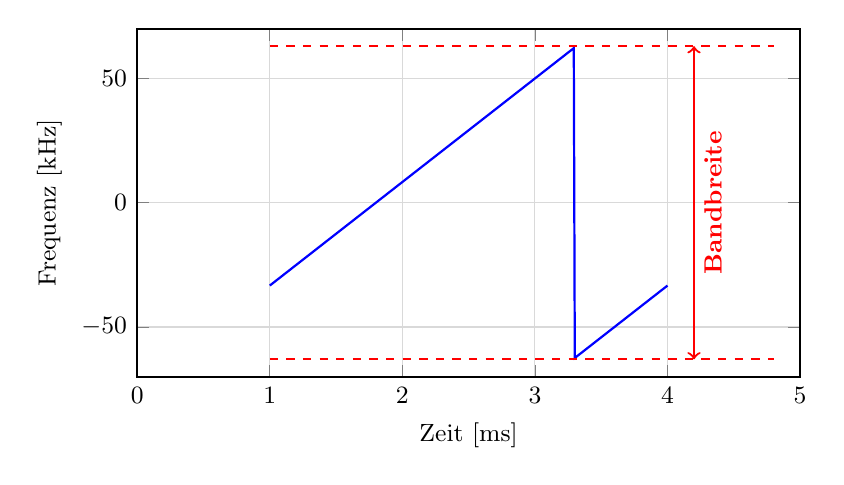
\begin{tikzpicture}
			\begin{axis}[
				width=10cm,
				height=6cm,
				xlabel={Zeit [ms]},
				ylabel={Frequenz [kHz]},
				xmin=0, xmax=5,
				ymin=-70, ymax=70,
				xtick={0,1,2,3,4,5},
				grid=both,
				every major grid/.style={gray!30},
				line width=0.8pt,
				tick label style={font=\small},
				label style={font=\small},
				unbounded coords=jump
				]
				% Chirp signal: linear sweep repeating every 2 ms
				\addplot[blue, thick, samples=400, domain=1:4]
				{ (mod(125*((x-0.3)/3),125))-62.5};
				
				\draw[dashed, red, thick] (axis cs:1,63) -- (axis cs:4.8,63);
				\draw[dashed, red] (axis cs:1,-63) -- (axis cs:4.8,-63);
				% Strzałka Bandbreite
				\draw[<->, thick, red] (axis cs:4.2,-63) -- (axis cs:4.2,63) node[midway, right, font=\small, rotate=90, below]{\textbf{Bandbreite}};
				
				
			\end{axis}
			
			
			%\fill[red!40, opacity=0.5] (axis cs:0,0) rectangle (axis cs:40,-4);
			%\draw[dashed, red] (1, 1) -- (5.5,50);
		\end{tikzpicture}
		\caption{Momentane Frequenz eines LoRa-Up-Chirps mit markierter Bandbreite (BW = 125 kHz)}
	\end{figure}

\subsection{Demodulation \label{lora:demodulation}}

	Die Demodulation der Chirp–Signale in LoRa basiert auf einem Korrelationsverfahren, bei dem das empfangene Signal mit den möglichen Chirp–Basisfunktionen verglichen wird, um das übertragene Symbol zu identifizieren \cite{Afisiadis:2020, Guo:2022}. Ein direkter Vergleich mit allen \( 2^{SF} \) möglichen Symbolen wäre jedoch rechnerisch sehr aufwendig, insbesondere bei gro{\ss}en Spreading–Faktoren (z.\,B. \( SF = 12 \Rightarrow 4096 \) mögliche Symbole).

	\medskip
	Daher verwendet LoRa ein effizienteres Verfahren, das die Korrelation indirekt bestimmt und sich auf eine einfache Multiplikation mit einem \emph{Down–Chirp} und eine anschlie{\ss}ende schnelle Fourier-Transformation (FFT) stützt. Durch diese sogenannte \emph{Dechirping}-Technik kann das empfangene Signal in den Frequenzbereich überführt werden, in dem die Symbolinformation als deutlicher Energie-Peak an einer bestimmten Position erscheint. Der Index dieses Peaks entspricht direkt dem gesendeten Symbolwert \cite{Vangelista:2017}.

	\medskip
	Das empfangene Signal kann beschrieben werden als
	\[
	r(t) = c_s(t) + w(t),
	\]
	wobei \( c_s(t) \) das übertragene Chirp-Signal und \( w(t) \) das additive wei{\ss}e Gau{\ss}sche Rauschen ist. Da das Symbol \( s \) im übertragenen Signal unbekannt ist, muss der Empfänger bestimmen, welches Chirp-Signal \( c_s(t) \) am besten mit dem Empfangssignal übereinstimmt \cite{Vangelista:2017}.
	
	\medskip
	\textbf{1) Dechirping-Schritt:}  
	Der Empfänger multipliziert das empfangene Signal mit einem \emph{Down-Chirp}, also einem Signal mit abnehmender Frequenz:
	\[
	d(t) = r(t) \cdot e^{-j 2 \pi \frac{t^2}{T_s^2}}.
	\]
	Durch diese Multiplikation heben sich die gegenläufigen Frequenzverläufe (Up- und Down-Chirp) gegenseitig auf, sodass das resultierende Signal \( d(t) \) eine \emph{konstante Frequenz} besitzt \cite{Vangelista:2017, Afisiadis:2020}.
	
	\begin{figure}[H]
		\centering
		
		% === UP CHIRP ===
		\begin{minipage}[t]{0.48\textwidth}
			\centering
			\textbf{(a) Up-Chirp} \\[3pt]
			\begin{tikzpicture}[
				every axis/.style={
					width=6cm,
					height=3.5cm,
					axis lines=middle,
					thick,
					xmin=0, xmax=1,
					ymin=0, ymax=1,
					xtick=\empty,
					ytick=\empty,
					ylabel style={rotate=-90},
					tick label style={font=\tiny},
				}
				]
				
				\begin{axis}[name=up_freq, ylabel={Frequenz}]
					\addplot[blue, thick, domain=0:0.9, samples=100] {x};
				\end{axis}
				
				\begin{axis}[
					name=up_amp,
					at=(up_freq.below south west),
					anchor=above north west,
					yshift=-0.5cm,
					ylabel={Amplitude},
					ymin=0, ymax=1,
					]
					\addplot[blue, thick, domain=0:1, samples=1000]
					{0.3*sin(deg(2*pi*(20*x^3))) + 0.5};
				\end{axis}
				
				\node[below=0cm of up_amp.south east, font=\small] {Zeit};
				
			\end{tikzpicture}
			
		\end{minipage}
		\hfill
		% === DOWN CHIRP ===
		\begin{minipage}[t]{0.48\textwidth}
			\centering
			\textbf{(b) Down-Chirp} \\[3pt]
			\begin{tikzpicture}[
				every axis/.style={
					width=6cm,
					height=3.5cm,
					axis lines=middle,
					thick,
					xmin=0, xmax=1,
					ymin=0, ymax=1,
					xtick=\empty,
					ytick=\empty,
					ylabel style={rotate=-90},
					tick label style={font=\tiny},
				}
				]
				
				\begin{axis}[name=down_freq, ylabel={Frequenz}]
					\addplot[blue, thick, domain=0:1, samples=100] {1 - x};
				\end{axis}
				
				\begin{axis}[
					name=down_amp,
					at=(down_freq.below south west),
					anchor=above north west,
					yshift=-0.5cm,
					ylabel={Amplitude},
					ymin=0, ymax=1,
					]
					\addplot[blue, thick, domain=0:1, samples=1000]
					{0.3*sin(deg(2*pi*(20*(1 - x)^3))) + 0.5};
				\end{axis}
				
				\node[below=0cm of down_amp.south east, font=\small] {Zeit};
				
			\end{tikzpicture}
		\end{minipage}
		\par\vspace{1cm} % przerwa pionowa (dowolna wartość)
		\begin{minipage}[t]{0.48\textwidth}
			\centering
			\textbf{Nach dem Downchirping} \\[3pt]
			\begin{tikzpicture}[
				every axis/.style={
					width=6cm,
					height=3.5cm,
					axis lines=middle,
					thick,
					xmin=0, xmax=1,
					ymin=0, ymax=1,
					xtick=\empty,
					ytick=\empty,
					ylabel style={rotate=-90},
					tick label style={font=\tiny},
				}
				]
				
				\begin{axis}[name=down_freq, ylabel={Frequenz}]
					\addplot[blue, thick, domain=0:1, samples=100] {0.5};
				\end{axis}
				
				\begin{axis}[
					name=down_amp,
					at=(down_freq.below south west),
					anchor=above north west,
					yshift=-0.5cm,
					ylabel={Amplitude},
					ymin=0, ymax=1,
					]
					\addplot[blue, thick, domain=0:1, samples=1000]
					{0.3*sin(deg(2*pi*(20*(1 - x)^1))) + 0.5};
				\end{axis}
				
				\node[below=0cm of down_amp.south east, font=\small] {Zeit};
				
			\end{tikzpicture}
			
		\end{minipage}
		
		\caption{Darstellung von Up- und Down-Chirps sowie des resultierenden Signals nach dem Downchirping im Chirp Spread Spectrum (CSS).}
	\end{figure}
	
	\medskip
	\textbf{2) FFT-Schritt:}  
	Anschlie{\ss}end wird auf das dechirpte Signal \( d(nT_s) \) eine diskrete Fourier-Transformation (DFT) angewendet.  
	Die DFT kann formal wie folgt ausgedrückt werden \cite{Vangelista:2017}:
	\[
	\tilde{D}_p = \sum_{k=0}^{N-1} d(nT_s + kT_s)\, e^{-j 2\pi pk/N}.
	\]
	Der Index \( p \), bei dem die spektrale Energie \( |\tilde{D}_p|^2 \) maximal ist, entspricht dem übertragenen Symbolwert:
	\[
	\hat{s} = \arg\max_p |\tilde{D}_p|^2.
	\]
	
	
	
	\begin{center}
		
\includegraphics[width=\linewidth]{LoRaAndLoRaWAN/FastFourierTransformation}
		\captionof{figure}{Normales Dechirping mit FFT; im Idealfall entsteht ein deutlicher Peak wie in (a3) \cite{Xu:2023}}
	\end{center}
	
	\medskip
	\textbf{Interpretation:}  
	Der Prozess des Dechirping wandelt den empfangenen Up-Chirp in ein Signal mit fester Frequenz um, deren Wert proportional zum Symbol ist. Die anschlie{\ss}ende FFT identifiziert diese Frequenz effizient, sodass das ursprüngliche Symbol bestimmt werden kann. Damit lässt sich das empfangene Symbol mit minimalem Rechenaufwand rekonstruieren.
	
	\medskip
	Dieser Mechanismus macht die LoRa-Demodulation extrem energieeffizient und robust: Anstatt \( 2^{SF} \) Korrelationen durchzuführen, genügt eine Multiplikation und eine FFT. Darüber hinaus sorgt das frequenzvariable Chirp-Signal dafür, dass Störungen und Mehrwegeffekte über das gesamte Band „gemittelt“ werden, was die Zuverlässigkeit der Übertragung weiter erhöht.
	
\section{LoRa-Paket}
	Jede über \ac{lora} übertragene Frame besitzt eine klar definierte Struktur, deren Gesamtlänge von der Anzahl der Symbole abhängt. Wie in der offiziellen Dokumentation von Semtech beschrieben \cite{Semtech:2015b}, besteht ein LoRa-Paket aus drei Hauptkomponenten: der Präambel, dem Header und der Payload.
	
	\begin{figure}[H]
		\centering
		\begin{tikzpicture}
			\loraframe
		\end{tikzpicture}
		\caption{Aufbau einer LoRa-Frame \cite{Semtech:2015b}}
	\end{figure}
	
	\begin{center}
		\begin{tikzpicture}
			\node[anchor=south west, inner sep=0] (image) at (0,0) {%
				
\includegraphics[width=\linewidth]{LoRaAndLoRaWAN/chirpsExample}};
			
			\begin{scope}[x={(image.south east)}, y={(image.north west)}]
				
				% preamble
				\draw[red, line width=1.3pt, dashed] (0.09,0.43) rectangle (0.35, 0.7);
				\draw[red, line width=2pt, <-, >=angle 60] (0.2,0.42) -- ++(-0.01,-0.18) node[below] {Preamble};
				
				\draw[red, line width=1.3pt, dashed] (0.355,0.43) rectangle (0.8, 0.7);
				\draw[red, line width=2pt, <-, >=angle 60] (0.6,0.42) -- ++(0.01,-0.18) node[below] {Header + Payload};
			\end{scope}
		\end{tikzpicture}
		\captionof{figure}{10 Aufwärts-Chirps und 2 Abwärts-Chirps, gefolgt von der Paylad \cite{Gao:2023}}
	\end{center}
\subsection{Preamble}
	Die Präambel dient der Erkennung des LoRa-Pakets und der Synchronisation des Empfängers mit dem eintreffenden Datensignal. 
	Sie besteht standardmä{\ss}ig aus einer 12 Symbole langen Sequenz - 10 up-chirps und 2 Down-chirps \cite{Semtech:2024, Gao:2023}.  Die chirps die, nach den 2 down-chirps folgen, sind payload.
	Innerhalb der Präambel befindet sich auch das sogenannte \emph{Sync Word}, das der Unterscheidung zwischen verschiedenen Netzwerken dient.  
	Empfänger verarbeiten nur Pakete mit demselben \emph{Sync Word}, wodurch sich z.\,B. LoRaWAN- und proprietäre LoRa-Netzwerke voneinander abgrenzen lassen \cite{Savaux:2021}.
	
\subsection{Header}
	Der Header enthält Metadaten über das nachfolgende Nutzsignal und kann in zwei unterschiedlichen Modi übertragen werden:
	
	\begin{itemize}
		\item \textbf{Explicit Header Mode (Standardmodus)}\\
		In diesem Modus wird ein kurzer Header mitgesendet, der folgende Informationen enthält:
		\begin{itemize}
			\item Länge der Payload (in Byte),
			\item verwendete \hyperref[lora:codingRate]{Codierungsrate},
			\item Vorhandensein einer optionalen zyklischen Redundanzprüfung (CRC) für die Payload.
		\end{itemize}
		Dieser Header besteht immer aus 8 Symbolen, wird mit der maximalen Fehlerkorrekturstufe (\(4/8\)) übertragen und besitzt eine eigene CRC \cite{Semtech:2024}.
		
		\item \textbf{Implicit Header Mode}\\
		In diesem Modus wird kein Header übertragen, wodurch die Paketlänge und damit die Übertragungszeit reduziert werden. Die Informationen über die Payload-Länge, Codierungsrate und CRC-Anwesenheit müssen in diesem Fall sowohl auf Sender- als auch auf Empfängerseite manuell identisch eingestellt werden \cite{Semtech:2024}.
	\end{itemize}
	
\subsection{Payload}
	Die Payload enthält die eigentlichen Nutzdaten (\(p\)~Bytes), die mit der im Header oder in der Registerkonfiguration angegebenen Codierungsrate übertragen werden. Am Ende der Payload kann optional eine CRC hinzugefügt werden, die zur Fehlererkennung dient \cite{Semtech:2024}.
	
\subsection{Time-on-Air}
	Die Gesamtdauer einer LoRa-Übertragung (\textit{Time on Air}) hängt von der Anzahl der Symbole ab, 
	aus denen sich die Frame zusammensetzt. Diese Beziehung lässt sich allgemein durch folgende Gleichung beschreiben:
	\[
	T_\text{Frame} = N_\text{Sym} \cdot T_s
	\]
	wobei \(N_\text{Sym}\) die Gesamtzahl der Symbole in der Frame und \(T_s\) die Symbolzeit bezeichnet.  
	Je nach \textit{Spreading Factor} (\(SF\)), \textit{Coding Rate} (\(CR\)) und \textit{Bandbreite} (\(BW\)) 
	ändert sich somit die Übertragungsdauer einer einzelnen LoRa-Frame \cite{Montagny:2022, Semtech:2015b}.
	
\subsection{Paketübertragung – Beispiel}

Bei einem Spreading Factor von \textbf{SF10} werden jeweils \textbf{10 Bits} zu einem Symbol zusammengefasst. Somit existieren \(2^{10} = 1024\) mögliche Symbolkombinationen, die jeweils durch ein charakteristisches Chirp-Signal übertragen werden. Jedes Symbol repräsentiert also eine eindeutige Bitfolge, die während der Übertragung nacheinander gesendet wird \cite{Montagny:2022}.

\begin{figure}[H]
	\centering
	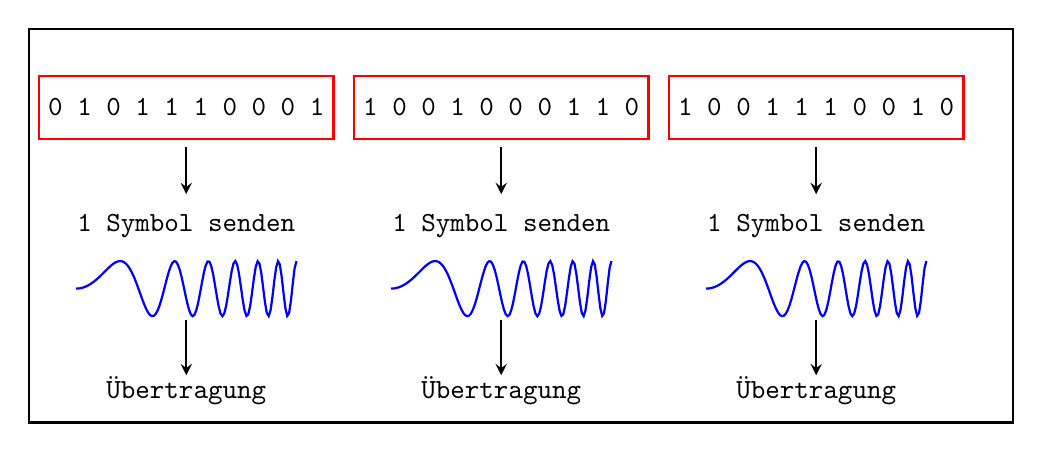
\begin{tikzpicture}[font=\ttfamily\bfseries, >=stealth, line width=0.8pt]
		
		\def\bitsA{0 1 0 1 1 1 0 0 0 1}
		\def\bitsB{1 0 0 1 0 0 0 1 1 0}
		\def\bitsC{1 0 0 1 1 1 0 0 1 0}
		
		\node[draw=red, thick, minimum width=3.3cm, minimum height=0.8cm, align=center] (b1) at (0,0) {\bitsA};
		\node[draw=red, thick, minimum width=3.3cm, minimum height=0.8cm, align=center] (b2) at (4,0) {\bitsB};
		\node[draw=red, thick, minimum width=3.3cm, minimum height=0.8cm, align=center] (b3) at (8,0) {\bitsC};
		
		\foreach \b/\x in {b1/0, b2/4, b3/8} {
			\draw[->, thick] (\x,-0.5) -- (\x,-1.1);
			\node[align=center] at (\x,-1.5) {1 Symbol senden};
			
			\draw[domain=0:2.8, samples=120, blue, variable=\t, shift={(\x-1.4,-2.3)}]
			plot ({\t}, {0.35*sin(deg(5*\t^2))});
			
			\draw[->, thick] (\x,-2.7) -- (\x,-3.4);
			\node[align=center] at (\x,-3.6) {Übertragung};
		}
		
		\draw[black, thick] (-2,-4) rectangle (10.5,1);
		
	\end{tikzpicture}
	\caption{Beispielhafte Darstellung der Paketübertragung bei SF10: 
		Zehn Bits werden zu einem Symbol zusammengefasst und nacheinander als Chirp-Signale übertragen 
		(\(2^{10} = 1024\) mögliche Symbole) \cite{Montagny:2022}.}
\end{figure}




